% Gerado automaticamente. No preambulo do documento use:
% \usepackage{pgfplots}
% \pgfplotsset{compat=1.18}
\definecolor{plotblue}{HTML}{2563EB}
\definecolor{plotorange}{HTML}{D97706}
\definecolor{plotgreen}{HTML}{059669}
\definecolor{plotpurple}{HTML}{7C3AED}
\definecolor{plotgray}{HTML}{374151}
\definecolor{plotred}{HTML}{DC2626}
\definecolor{plotteal}{HTML}{0F766E}
\definecolor{plotslate}{HTML}{64748B}

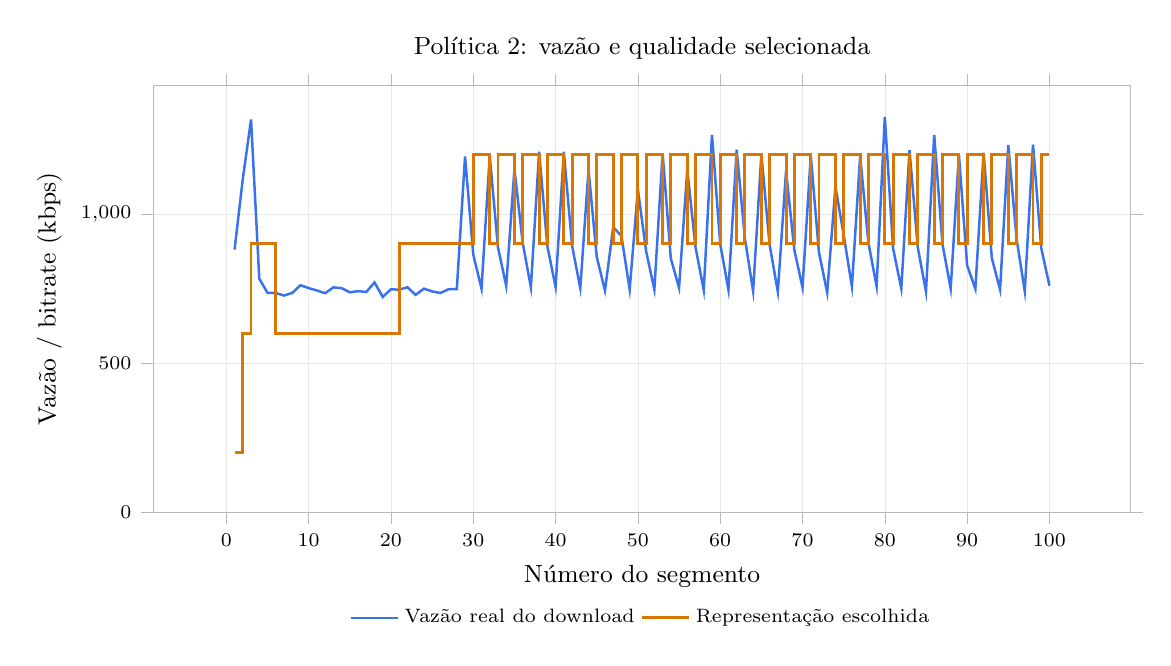
\begin{tikzpicture}
\begin{axis}[
    title={Política 2: vazão e qualidade selecionada},
    xlabel={Número do segmento},
    ylabel={Vazão / bitrate (kbps)},
    width=14cm,
    height=7cm,
    grid=major,
    grid style={line width=.12pt, draw=gray!18},
    axis line style={draw=gray!55},
    tick style={draw=gray!55},
    tick align=outside,
    title style={font=\small},
    label style={font=\small},
    tick label style={font=\scriptsize},
    legend cell align={left},
    legend style={at={(0.5,-0.20)}, anchor=north, legend columns=3, draw=none, font=\scriptsize},
    ymin=0,
    ymax=1431.25
]
\addplot+[plotblue, line width=0.9pt, mark=none, opacity=0.9] coordinates {
(1,880.71)
(2,1117.29)
(3,1317)
(4,783.19)
(5,735.22)
(6,734.76)
(7,726.35)
(8,734.94)
(9,761)
(10,751.33)
(11,743.3)
(12,734.17)
(13,753.68)
(14,751.23)
(15,737.19)
(16,741.02)
(17,738.21)
(18,770.34)
(19,721.84)
(20,747.31)
(21,745.99)
(22,754.15)
(23,728.45)
(24,749.44)
(25,740.15)
(26,734.95)
(27,747.43)
(28,747.8)
(29,1192.69)
(30,863.63)
(31,749.34)
(32,1194.82)
(33,887.55)
(34,758.78)
(35,1150.81)
(36,903.75)
(37,753.62)
(38,1208.59)
(39,891.9)
(40,755.07)
(41,1208.62)
(42,894.43)
(43,751.06)
(44,1149.04)
(45,855.79)
(46,743.22)
(47,955.83)
(48,926.17)
(49,746.73)
(50,1082.37)
(51,874.4)
(52,746.79)
(53,1203.77)
(54,850.8)
(55,752.35)
(56,1148.25)
(57,888.44)
(58,744.46)
(59,1265.26)
(60,899.51)
(61,745.32)
(62,1215.72)
(63,917.82)
(64,740.9)
(65,1200.35)
(66,897.24)
(67,738.79)
(68,1144.52)
(69,880.54)
(70,753.17)
(71,1195.25)
(72,870.69)
(73,736.11)
(74,1091.62)
(75,929.95)
(76,756.48)
(77,1195.46)
(78,904.22)
(79,757.09)
(80,1325.23)
(81,885.12)
(82,749.69)
(83,1213.82)
(84,888.57)
(85,739.46)
(86,1264.92)
(87,899.68)
(88,749.4)
(89,1198.72)
(90,827.33)
(91,748.82)
(92,1205.41)
(93,851.93)
(94,745.98)
(95,1231.27)
(96,918.13)
(97,740.93)
(98,1232.75)
(99,885.96)
(100,759.54)
};
\addlegendentry{Vazão real do download}
\addplot+[plotorange, const plot, line width=1.05pt, mark=none] coordinates {
(1,200)
(2,600)
(3,900)
(4,900)
(5,900)
(6,600)
(7,600)
(8,600)
(9,600)
(10,600)
(11,600)
(12,600)
(13,600)
(14,600)
(15,600)
(16,600)
(17,600)
(18,600)
(19,600)
(20,600)
(21,900)
(22,900)
(23,900)
(24,900)
(25,900)
(26,900)
(27,900)
(28,900)
(29,900)
(30,1200)
(31,1200)
(32,900)
(33,1200)
(34,1200)
(35,900)
(36,1200)
(37,1200)
(38,900)
(39,1200)
(40,1200)
(41,900)
(42,1200)
(43,1200)
(44,900)
(45,1200)
(46,1200)
(47,900)
(48,1200)
(49,1200)
(50,900)
(51,1200)
(52,1200)
(53,900)
(54,1200)
(55,1200)
(56,900)
(57,1200)
(58,1200)
(59,900)
(60,1200)
(61,1200)
(62,900)
(63,1200)
(64,1200)
(65,900)
(66,1200)
(67,1200)
(68,900)
(69,1200)
(70,1200)
(71,900)
(72,1200)
(73,1200)
(74,900)
(75,1200)
(76,1200)
(77,900)
(78,1200)
(79,1200)
(80,900)
(81,1200)
(82,1200)
(83,900)
(84,1200)
(85,1200)
(86,900)
(87,1200)
(88,1200)
(89,900)
(90,1200)
(91,1200)
(92,900)
(93,1200)
(94,1200)
(95,900)
(96,1200)
(97,1200)
(98,900)
(99,1200)
(100,1200)
};
\addlegendentry{Representação escolhida}
\end{axis}
\end{tikzpicture}
